% !TeX root = ../tesi.tex
% !TeX encoding = UTF-8
% !TeX spellcheck = it_IT

\chapter{Pipeline, dataset e filtraggio}
\label{chap:dataset}

In questo capitolo descrivo come collego le immagini politiche, le informazioni ricavate dalla loro elaborazione e l'engagement dei post. Presento prima l'architettura della pipeline, specificando gli input, i passaggi e gli output (Sezione~\ref{sec:pipeline-architettura}). Descrivo poi il dataset (Sezione~\ref{sec:materiali-dataset}), la misura di engagement (Sezione~\ref{sec:pipeline-engagement}) e il filtraggio con cui costruisco il campione (Sezione~\ref{sec:dataset-selezione}). Ne discuto infine i limiti (Sezione~\ref{sec:dataset-limiti}).

Nel Capitolo~\ref{chap:localizzazione-descrizione} presento l'integrazione di TruFor, il test preliminare, il mascheramento e la descrizione delle regioni sospette. Nel Capitolo~\ref{chap:caratteristiche-visive} descrivo il ramo che estrae le caratteristiche visive dall'immagine intera.

\section{Architettura della pipeline}
\label{sec:pipeline-architettura}

Organizzo il sistema secondo il flusso della Figura~\ref{fig:pipeline-generale}. Parto dai post e dalle immagini associate. Ricavo il punteggio globale di TruFor, il testo delle regioni sospette e le caratteristiche visive dell’immagine intera, poi ne studio l’associazione con l’engagement.

Raccolgo le dipendenze Python e le relative versioni nel file \path{requirements.txt}. Il file permette di predisporre l'ambiente di esecuzione mediante il comando \texttt{pip install -r requirements.txt}.

Il progetto può essere eseguito su diversi sistemi operativi, purché l'ambiente supporti le dipendenze richieste e la creazione dei collegamenti simbolici usati dalla pipeline. L'esecuzione si adatta anche a hardware diversi: i modelli possono usare GPU NVIDIA tramite CUDA, GPU Apple Silicon tramite MPS oppure la CPU in assenza di accelerazione compatibile. La disponibilità dell'accelerazione dipende dall'hardware e dall'installazione di PyTorch; le risorse della macchina incidono sui tempi di elaborazione e sulle dimensioni dei gruppi di immagini elaborabili.

\subsection{Input e unità di analisi}
\label{subsec:pipeline-input}

La pipeline riceve i metadati dei post e i file multimediali scaricati dai relativi allegati. Dai metadati ricavo l'identificatore del post, il collegamento all'immagine e il punteggio di engagement. Attraverso il filtraggio associo ogni immagine selezionata a un solo post di riferimento. L'\emph{unità di analisi} è quindi un'immagine con la misura di engagement della pubblicazione a cui la collego.

Uso i pixel dell'immagine per ricavare le informazioni sul contenuto e sull'aspetto visivo. Mantengo l'engagement come risposta osservata con cui confronto queste informazioni. I modelli forensi e di descrizione ricevono le immagini, senza usare il punteggio di engagement per localizzare o descrivere le regioni sospette.

\subsection{Passaggi e collegamenti tra i componenti}
\label{subsec:pipeline-passaggi}

Il ramo delle caratteristiche visive non dipende dal mascheramento. Posso quindi confrontare le informazioni sul contenuto delle regioni selezionate con quelle sull'aspetto complessivo dell'immagine.

Riassumo nella Tabella~\ref{tab:pipeline-passaggi} gli input e gli output dei componenti. Le analisi finali usano le informazioni raccolte per studiare le associazioni con l'engagement e classificare i post rispetto alle aspettative dell'account. Confronto il solo punteggio TruFor con le rappresentazioni arricchite e interpreto le previsioni del modello sulle parole.

\begin{table}[htbp]
    \centering
    \small
    \caption{Input e output dei passaggi della pipeline. Le caratteristiche visive derivano dall'immagine intera; la descrizione testuale deriva dal contenuto conservato dalla maschera.}
    \label{tab:pipeline-passaggi}
    \begin{tabular}{@{}>{\raggedright\arraybackslash}p{0.22\linewidth}>{\raggedright\arraybackslash}p{0.32\linewidth}>{\raggedright\arraybackslash}p{0.39\linewidth}@{}}
        \toprule
        Passaggio & Input & Output \\
        \midrule
        Filtraggio & Metadati e file multimediali & Immagini associate a un post e al suo engagement. \\
        \addlinespace
        TruFor~\cite{Guillaro_2023_CVPR} & Immagine intera & Punteggio globale e mappe delle anomalie e di confidenza. \\
        \addlinespace
        Mascheramento & Immagine e mappe TruFor & Immagine con le regioni selezionate su sfondo nero. \\
        \addlinespace
        Descrizione & Immagine mascherata & Testo da BLIP~\cite{pmlr-v162-li22n} e OCR~\cite{easyocr_software} normalizzato e unito, oppure \texttt{nomask} in assenza di una descrizione utilizzabile. \\
        \addlinespace
        Caratteristiche visive & Immagine intera & Vettore di 19 misure. \\
        \addlinespace
        Analisi dell'engagement & Punteggio TruFor, testo vettorizzato, caratteristiche visive ed engagement & Associazioni statistiche, previsioni, misure di prestazione e spiegazioni. \\
        \bottomrule
    \end{tabular}
\end{table}

\subsection{Output condivisi e tracciabilità}
\label{subsec:pipeline-output}

Raccolgo le informazioni in \path{dataset_filtered.csv}. Il filtraggio crea una riga per immagine, con l'identificatore del post, il punteggio di engagement e il campo \texttt{filename}. Uso quest'ultimo per associare gli output successivi alla riga corrispondente. Aggiungo il punteggio \texttt{trufor\_score}, le caratteristiche visive e il testo \texttt{anomaly\_txt}.

Conservo gli output intermedi nella cartella di lavoro \path{scripts/temp/}. La cartella \path{scripts/temp/images/} mantiene i collegamenti agli originali selezionati. I file \texttt{.npz} in \path{scripts/temp/npz/} contengono le mappe di TruFor; le immagini in \path{scripts/temp/masked/} mostrano il contenuto fornito ai modelli di descrizione. Il campo \texttt{filename} collega ogni descrizione e punteggio TruFor alla corrispondente immagine originale.

Centralizzo percorsi e parametri in \path{scripts/config.py}. Mantengo separati il codice di TruFor e gli script che gestiscono filtraggio, caratteristiche visive, mascheramento, descrizione e analisi. Uso i pesi preaddestrati di TruFor, BLIP ed EasyOCR; stimo sul campione i modelli per l'associazione con l'engagement. Le regole con cui costruisco il campione e distinguo le sue diverse numerosità sono descritte nella Sezione~\ref{sec:dataset-selezione}.

\section{Dataset}
\label{sec:materiali-dataset}

\subsection{Origine dei dati e contesto della raccolta}
\label{subsec:dataset-origine}

Utilizzo una raccolta di contenuti pubblici di comunicazione politica pubblicati su Facebook e Instagram tra il 15 maggio e il 14 agosto 2024. L'intervallo comprende il periodo delle elezioni europee del 2024, tenutesi tra il 6 e il 9 giugno. I dati provengono da CrowdTangle e comprendono i metadati dei post e i materiali multimediali scaricati dai collegamenti agli allegati.

La disponibilità congiunta di immagini e misure di engagement motiva l'adozione di questo dataset. Posso associare a ciascuna immagine le informazioni prodotte dalla \emph{pipeline}, cioè dalla sequenza di elaborazioni automatiche, e confrontarle con la risposta degli utenti alla pubblicazione. La raccolta può comprendere sia inserzioni sponsorizzate sia resoconti delle attività dei politici.

\subsubsection{CrowdTangle e i dati disponibili}
\label{subsubsec:dataset-crowdtangle}

Il \emph{Codebook}, la documentazione tecnica di \emph{CrowdTangle}, descrive il servizio come una piattaforma di analisi dei contenuti pubblici. Mette a disposizione metadati e contatori di interazione, rilevati dalla pubblicazione fino all'interrogazione. La copertura dipende dagli account monitorati; per Facebook, la documentazione esclude i contenuti con restrizioni di pubblico imposte tramite strumenti di targeting~\cite{DVN/SCCQYD_2019}.

La raccolta è stata effettuata tramite l'API di CrowdTangle, con salvataggio dei metadati dei post e download dei relativi allegati. CrowdTangle permetteva di organizzare gli account in liste interne alla piattaforma. La lista dei candidati italiani era stata curata da sociologi della Sapienza. Considero i 66 account presenti nel dataset, 28 Facebook e 38 Instagram, come un sottoinsieme di una lista più ampia e descrivo il campione sulla base dei metadati disponibili.

Assumo come punto di partenza l’archivio disponibile, composto da 1.357 post di 66 account. La documentazione della raccolta non permette di verificarne la completezza rispetto alla lista iniziale. Nella Sezione~\ref{sec:dataset-selezione} descrivo i filtri che applico per costruire il campione analizzato.

\subsection{Composizione e struttura del dataset}
\label{subsec:dataset-struttura}

Il dataset originale contiene 1.357 post pubblicati da 66 account. La Tabella~\ref{tab:dataset-piattaforme} ne riporta la distribuzione per piattaforma e la confronta con quella delle immagini nel campione filtrato, definito nella Sezione~\ref{sec:dataset-selezione}.

\begin{table}[htbp]
    \centering
    \caption{Composizione per piattaforma. Nel campione filtrato ogni immagine è associata a un solo post di riferimento.}
    \label{tab:dataset-piattaforme}
    \begin{tabular}{lrr}
        \toprule
        Piattaforma & Post originali & Immagini nel campione filtrato \\
        \midrule
        Facebook  & 521   & 386   \\
        Instagram & 836   & 826   \\
        \midrule
        Totale    & 1.357 & 1.212 \\
        \bottomrule
    \end{tabular}
\end{table}

L'archivio comprende i metadati, raccolti in \path{crowdtangle.jsonl}, e una cartella di contenuti multimediali. Il formato adottato per i primi è \emph{JSON Lines}: ogni riga contiene un oggetto \emph{JSON}, ossia una struttura di campi e valori che descrive un post. La cartella \path{crowdtangle_media/} contiene 1.441 file: 1.192 con estensione \texttt{.jpg}, 82 \texttt{.heic}, 20 \texttt{.webp}, 98 \texttt{.mp4}, 7 \texttt{.mpd} e 42 senza estensione.

Le liste degli allegati nei metadati citano complessivamente 1.466 elementi, di cui 1.348 fotografie e 118 video. Ho quindi tre quantità: i post raccolti, gli allegati citati e i file presenti su disco. Un post può avere più allegati; nella Sezione~\ref{sec:dataset-selezione} specifico come seleziono quello da analizzare e verifico la disponibilità del file corrispondente.

Per studiare la relazione tra contenuti visivi ed engagement, associo ciascuna immagine all’indice di engagement della pubblicazione di riferimento. A questo scopo seleziono i metadati riportati nella Tabella~\ref{tab:dataset-campi} e mantengo inalterato il dataset originale.

\bigskip\noindent
\begin{minipage}{\linewidth}
    \centering
    \captionsetup{type=table}
    \caption{Campi utilizzati per associare un post alla sua immagine e al risultato di engagement. I campi \texttt{type}, \texttt{url} e \texttt{full} appartengono all'allegato selezionato nella lista \texttt{media}~\cite{DVN/SCCQYD_2019}.}
    \label{tab:dataset-campi}
    \begin{tabular}{@{}lp{0.69\textwidth}@{}}
        \toprule
        Campo & Significato \\
        \midrule
        \texttt{id} & Identificatore del post di riferimento. \\
        \texttt{score} & Punteggio di engagement. \\
        \texttt{media} & Lista degli allegati. Prendo il primo elemento. \\
        \texttt{type} & Tipo dell'allegato: seleziono il tipo \texttt{photo}. \\
        \texttt{url}, \texttt{full} & Campi dell'allegato che contengono il collegamento al file. Uso \texttt{url} o in alternativa \texttt{full}. \\
        \bottomrule
    \end{tabular}
\end{minipage}
\bigskip

\section{Engagement e classi di riferimento}
\label{sec:pipeline-engagement}

\subsection{Definizione del punteggio di engagement}
\label{subsec:dataset-engagement}

Sfrutto come misura dell'engagement il campo \texttt{score}, basato sulla metrica \emph{overperforming} di CrowdTangle. Questa metrica confronta le interazioni osservate con un benchmark di riferimento, relativo a post dello stesso account, dello stesso tipo e con un tempo trascorso dalla pubblicazione comparabile.

Il benchmark considera gli ultimi 100 post comparabili. Per ciascun tipo di interazione, CrowdTangle ordina i valori, elimina i 25 maggiori e i 25 minori e calcola la media dei 50 centrali. Il calcolo prevede inoltre soglie minime per limitare l'instabilità dovuta a conteggi piccoli.

Indico con $c_i$ il punteggio del post associato all'immagine $i$, con $I_i$ le interazioni osservate, sommate nella configurazione predefinita, con $B_i$ il benchmark corrispondente e con $\tau$ la soglia minima di interazioni. Per $B_i>0$ e $I_i>0$, il calcolo distingue quattro casi:
\begin{equation}
    c_i =
    \begin{cases}
        \dfrac{I_i}{B_i} & \text{se } I_i \geq B_i \text{ e } I_i \geq \tau, \\[6pt]
        \dfrac{I_i}{\tau} & \text{se } I_i \geq B_i \text{ e } I_i < \tau, \\[6pt]
        -\dfrac{B_i}{I_i} & \text{se } I_i < B_i \text{ e } I_i \geq \tau, \\[6pt]
        -\dfrac{B_i-I_i}{B_i} & \text{se } I_i < B_i \text{ e } I_i < \tau.
    \end{cases}
    \label{eq:dataset-overperforming}
\end{equation}
Il Codebook indica inoltre $c_i=-2B_i$ in assenza di interazioni. La soglia $\tau$ dipende dalla piattaforma e dal tipo di interazione: ad esempio, è pari a 5 per i like e a 2 per i commenti su Facebook e Instagram.

I primi due casi riguardano prestazioni pari o superiori al benchmark; gli ultimi due esprimono una prestazione inferiore tramite il segno negativo. Quando $I_i\geq\tau$, ad esempio, il doppio delle interazioni attese corrisponde a $2$, mentre la metà a $-2$. Con pochi eventi intervengono invece le correzioni indicate nella formula: uno score vicino allo zero non implica necessariamente che le interazioni siano vicine al benchmark.

\subsection{Binarizzazione del punteggio di engagement}
\label{subsec:dataset-binarizzazione}

Per le analisi di classificazione trasformo $c_i$ in una variabile binaria $y_i$. Nella configurazione utilizzata escludo i casi con score nell'intervallo $[-0{,}5;\,0{,}5]$, estremi inclusi. Per le osservazioni rimanenti definisco:
\begin{equation}
    y_i =
    \begin{cases}
        1 & \text{se } c_i > 0{,}5, \\
        0 & \text{se } c_i < -0{,}5.
    \end{cases}
    \label{eq:dataset-target}
\end{equation}
Come si osserva nella Figura~\ref{fig:dataset-istogramma}, l'intervallo centrale presenta poche osservazioni rispetto alle concentrazioni ai lati dello zero. Questa esclusione rimuove 16 post su 1.212, l'1,32\%.

Questa scelta circoscrive il confronto ai post con punteggi più distanti dallo zero, usato come soglia di separazione tra le due classi. Applico questa esclusione solo alle analisi di classificazione. Le statistiche descrittive del campione filtrato comprendono invece tutte le osservazioni, incluse quelle con indice vicino o uguale a zero. Le etichette $y_i$ indicano se la risposta degli utenti supera o meno le aspettative.

\section{Filtraggio e costruzione del campione}
\label{sec:dataset-selezione}

Per realizzare la corrispondenza prevista dall'unità di analisi definita nella Sottosezione~\ref{subsec:pipeline-input}, applico due passaggi: seleziono le pubblicazioni con una prima fotografia disponibile su disco e risolvo le associazioni multiple tra uno stesso file e più post.

\subsection{Selezione dei post e associazione ai file}
\label{subsec:dataset-filtraggio}

Costruisco un indice dei media presenti su disco tramite lo script \path{scripts/filter.py}. Per ciascun file leggo il nome senza estensione, che corrisponde già all'\emph{hash} dell'URL da cui è stato scaricato. L'hash è un identificatore che si ottiene applicando la funzione SHA-256 all'URL; nella configurazione corrente sfrutto tutti i suoi 64 caratteri esadecimali.

Considero i post per cui è disponibile la misura di engagement e che hanno come primo allegato una fotografia. Leggo il collegamento dal campo \texttt{url} o in alternativa \texttt{full}. Calcolo l'hash dell'URL e lo cerco nell'indice locale. Conservo l'osservazione soltanto se trovo un unico file corrispondente. Ignoro gli eventuali allegati successivi, inclusi i video.

Se più post rimandano allo stesso media, conservo quello con il punteggio maggiore. In caso di parità conservo il primo incontrato nell'archivio. Ottengo così una sola osservazione per media. Questa procedura riconosce le ripetizioni attraverso il collegamento all'allegato: immagini visivamente identiche disponibili a indirizzi diversi possono mantenere identificatori distinti, e quindi apparire più volte tra le immagini selezionate.

\subsection{Numerosità e struttura del campione filtrato}
\label{subsec:dataset-campione-filtrato}

La Tabella~\ref{tab:dataset-selezione} riporta il numero di osservazioni escluse e mantenute ad ogni passaggio del filtraggio. La riduzione del campione dipende soprattutto dal requisito che il primo allegato sia una fotografia.

\begin{table}[htbp]
    \centering
    \caption{Costruzione del campione filtrato. I criteri sono applicati in sequenza; ogni esclusione viene conteggiata una sola volta.}
    \label{tab:dataset-selezione}
    \begin{tabular}{@{}p{0.64\textwidth}rr@{}}
        \toprule
        Passaggio & Esclusioni & Rimanenti \\
        \midrule
        Archivio originale & -- & 1.357 \\
        Disponibilità dello score & 0 & 1.357 \\
        Presenza di almeno un allegato & 9 & 1.348 \\
        Primo allegato di tipo \texttt{photo} & 118 & 1.230 \\
        Presenza del file locale & 12 & 1.218 \\
        Un solo file locale per identificatore & 0 & 1.218 \\
        Un solo post per identificatore di file & 6 & 1.212 \\
        \bottomrule
    \end{tabular}
\end{table}

Il filtro produce un documento \emph{CSV}, cioè una tabella di valori separati da virgole, con le colonne \texttt{id}, \texttt{crowdtangle\_score} e \texttt{filename}. Ogni riga identifica un post, il suo score e il collegamento alla fotografia associata. La cartella \path{scripts/temp/images/} contiene i collegamenti ai file selezionati. La pipeline accede agli originali tramite questi collegamenti e conserva l'archivio di partenza inalterato.

Distinguo il risultato del filtraggio dalla tabella arricchita disponibile in \path{dataset_filtered.csv}, che contiene anche i punteggi di manipolazione, le descrizioni e le caratteristiche visive prodotte dalle elaborazioni successive. Quest'ultima comprende 1.211 osservazioni: una delle 1.212 immagini selezionate dal filtro è un PNG di dimensioni $1 \times 1$ pixel, che viene scartato nelle analisi successive. I due archivi coincidono per identificatore del post e misura di engagement sulle osservazioni comuni. Le statistiche della Sottosezione~\ref{subsec:dataset-statistiche} si riferiscono alle 1.212 immagini selezionate; la numerosità delle analisi successive dipende anche dalla disponibilità delle informazioni richieste da ciascun modello.

\subsection{Statistiche descrittive del campione}
\label{subsec:dataset-statistiche}

Nel campione filtrato, 386 casi provengono da Facebook e 826 da Instagram, rispettivamente il 31,8\% e il 68,2\% del totale. Rimangono rappresentati tutti i 66 account dell'archivio originale. Le statistiche di engagement si basano sulla misura associata a ciascuna pubblicazione di riferimento.

La Tabella~\ref{tab:dataset-statistiche} mostra che la media del punteggio di engagement, $-3{,}383$, è inferiore alla mediana, $-0{,}736$. La differenza, evidenziata dal $-8{,}717$ del coefficiente di asimmetria, indica la maggior presenza di osservazioni nella coda negativa: il minimo è $-304$, mentre il massimo è $81{,}75$.

Per individuare le osservazioni estreme ricorro alle soglie di Tukey. Indico con $Q_1$ e $Q_3$ il primo e il terzo \emph{quartile}, ossia le soglie al di sotto delle quali si colloca rispettivamente il 25\% e il 75\% delle osservazioni. Definisco l'intervallo interquartile come $\mathrm{IQR}=Q_3-Q_1$ e considero estremi gli score inferiori a $Q_1-1{,}5\,\mathrm{IQR}$ o superiori a $Q_3+1{,}5\,\mathrm{IQR}$~\cite{tukey1977exploratory}. Le soglie sono pari a circa $-7{,}895$ e $7{,}578$: 127 osservazioni, il 10,5\% del totale, si trovano al di fuori di questo intervallo. Mantengo queste osservazioni nell'analisi, perché il superamento delle soglie descrive la loro posizione nella distribuzione e non indica un errore nei dati.

\begin{table}[htbp]
    \centering
    \caption{Statistiche della misura di engagement sulle 1.212 immagini selezionate, prima dell'esclusione dei casi prossimi allo zero. I valori estremi sono individuati con le soglie di Tukey~\cite{tukey1977exploratory}.}
    \label{tab:dataset-statistiche}
    \begin{tabular}{lr}
        \toprule
        Statistica & Valore \\
        \midrule
        Media & $-3{,}383$ \\
        Mediana & $-0{,}736$ \\
        Deviazione standard & $23{,}506$ \\
        Minimo & $-304{,}000$ \\
        Primo quartile ($Q_1$) & $-2{,}092$ \\
        Terzo quartile ($Q_3$) & $1{,}776$ \\
        Massimo & $81{,}750$ \\
        Coefficiente di asimmetria & $-8{,}717$ \\
        Osservazioni oltre le soglie di Tukey & 127 (10,5\%) \\
        \bottomrule
    \end{tabular}
\end{table}

La Figura~\ref{fig:dataset-istogramma} mostra un istogramma della misura di engagement associata alle 1.212 immagini del campione filtrato. Per rendere leggibile la parte centrale della distribuzione, applico il \emph{clipping} solo nella rappresentazione grafica: riporto gli score inferiori a $-7{,}895$ sulla soglia inferiore e quelli superiori a $7{,}578$ sulla soglia superiore. Ad esempio, rappresento lo score $-304$ nella barra che contiene la soglia $-7{,}895$. Le barre ai bordi includono quindi anche le 127 osservazioni estreme. Nella parte centrale emergono due concentrazioni, ai lati dello zero, separate da una zona con poche osservazioni. La Figura~\ref{fig:dataset-boxplot} presenta un diagramma a scatola, o \emph{box plot}, della distribuzione originale, che mostra anche l'estensione della coda negativa.

\bigskip\noindent
\begin{minipage}{\linewidth}
    \centering
    \captionsetup{type=figure}
    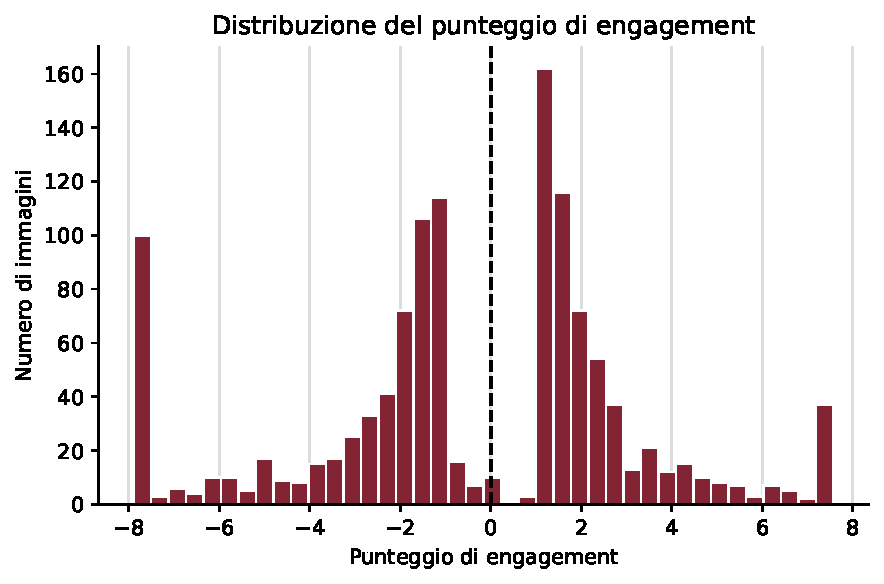
\includegraphics[width=0.7\textwidth]{engagement_istogramma.pdf}
    \caption{Istogramma del punteggio di engagement sulle 1.212 immagini selezionate. I 127 valori esterni alle soglie di Tukey~\cite{tukey1977exploratory} sono riportati sulle rispettive soglie e contribuiscono alle barre ai bordi. La linea tratteggiata indica lo zero.}
    \label{fig:dataset-istogramma}
\end{minipage}
\bigskip

\begin{figure}[htbp]
    \centering
    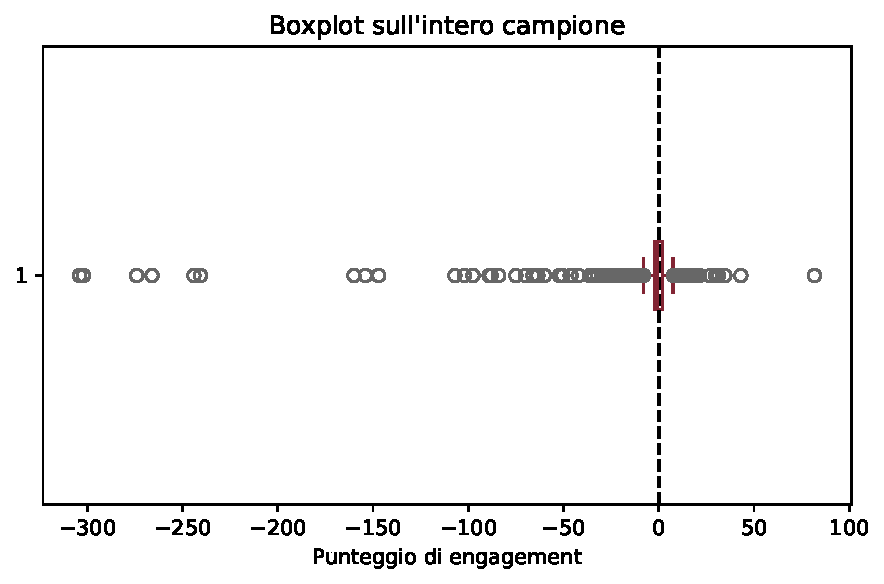
\includegraphics[width=0.7\textwidth]{engagement_boxplot.pdf}
    \caption{Box plot del punteggio di engagement sulle 1.212 immagini selezionate. La scatola rappresenta l'intervallo interquartile, la linea interna la mediana e i punti oltre i baffi i valori estremi~\cite{tukey1977exploratory}. La linea tratteggiata indica lo zero.}
    \label{fig:dataset-boxplot}
\end{figure}

\newpage
Dopo il filtraggio conto 584 score positivi, 618 negativi e 10 nulli. L'esclusione dell'intervallo $[-0{,}5;\,0{,}5]$ rimuove 16 osservazioni e lascia 1.196 esempi: 584 con prestazioni superiori alle aspettative e 612 con prestazioni inferiori. Applico la stessa regola alla tabella arricchita con le informazioni prodotte dalle elaborazioni successive, di 1.211 righe, e le osservazioni diventano 1.195, suddivise in 583 esempi con engagement superiore alle aspettative e 612 con engagement inferiore alle aspettative. Questa distinzione rende esplicita la differenza tra il campione descritto qui e quello riportato nelle analisi di classificazione archiviate.

\section{Limiti del dataset}
\label{sec:dataset-limiti}

La raccolta riguarda due piattaforme, 66 account in un intervallo di tre mesi. Questi confini delimitano il caso di studio. La prevalenza di Instagram, 68,2\% del totale dei post filtrati, e l'assenza di un protocollo completo di estrazione impediscono di considerare i dati selezionati una rappresentazione esaustiva dell'intera comunicazione politica online. L'estensione dei risultati ad altre campagne, periodi o ambiti del marketing richiede una verifica su nuove raccolte.

La scelta della prima immagine riduce ogni post a una sola componente visiva. La misura di engagement riguarda però il post nel suo complesso, che può includere testo e altri allegati. Le associazioni osservate coinvolgono quindi un contesto comunicativo che la rappresentazione dell'immagine descrive solo in parte.

Quando più post condividono il collegamento a un media, la selezione basata sull’indice di engagement privilegia per costruzione la prestazione più alta tra le occorrenze disponibili. Inoltre, il confronto degli identificatori dei file non elimina tutte le possibili ripetizioni visive. Queste due proprietà vanno considerate quando si interpreta la distribuzione della misura di engagement e quando si valuta l'indipendenza delle osservazioni.

Infine, l'engagement misura interazioni e non identifica direttamente consenso politico, persuasione o intenzione di voto. Il riferimento allo storico dell'account rapporta la misura alle sue prestazioni abituali, ma non permette di stabilire se una scelta visiva determina un cambiamento nelle interazioni. Utilizzo quindi il dataset per studiare le associazioni tra caratteristiche visive ed engagement e valutare quanto queste caratteristiche aiutano a prevederlo.
